\section{Digitalização de assinatura}

Digitalização de assinatura é um dos ramos da autenticação biométrica,
especificamente
na area de autenticação biométrica comportamental.

Segundo~\textcite{navaz2016}, para garantir a segurança e o controle na
identificação
biométrica de uma pessoa, é comum a necessidade de equipamentos, sensores ou
dispositivos específicos.
No entanto, a autenticação biométrica por meio de assinaturas requer apenas uma
caneta e papel.

Para determinar se uma assinatura é original ou falsa, é necessário obter uma
amostra da assinatura (seja de uma imagem digitalizada ou diretamente do
assinante)
e extrair características da imagem para compará-las a um banco de dados.
Por fim, é utilizado um classificador de algum tipo\cite{dewangan2015}.
\newpage

\begin{figure}[h!]
    \caption[Arquitetura de um sistema de autenticação via assinatura]
    {A arquitetura de um sistema baseado em assinatura manuscrita para
    registro e autenticação de usuários}
    \begin{adjustbox}{width=0.8\columnwidth, center}
        \begin{tikzpicture}[
            l/.style={
                draw, rectangle,
                fill=yellow!20,
                minimum width=5cm,
                minimum height=12cm
            },
            r/.style={
                draw, rectangle,
                fill=green!20,
                minimum width=5cm,
                minimum height=12cm
            },
            c/.style={
                opacity=.3,
                very thick,
                draw, rectangle,
                rounded corners,
                fill=black,
            },
            s/.style={
                very thick,
                draw, rectangle,
                fill=blue!20,
                draw=blue!70,
                text width=2cm,
                align=center
            },
            db/.style={cylinder,
            draw=blue!70,
            very thick,
            cylinder uses custom fill,
            cylinder body fill=blue!30,
            cylinder end fill=blue!20,
            aspect=0.25,
            shape border rotate=90,
            height=3cm,
            text width=2.5cm,
            align=center
            },
            t/.style={
                isosceles triangle,
                rotate=-90,
                very thick,
                draw=blue!70,
                fill=blue!20,
            }
        ]
            
            \node[s, text width=3cm](interface1) at (2.5, 7){Interface do usuário};
            \node[t, yshift=0.2cm, xshift=-0.3cm][below=0.5cm of interface1];
            
            \node[xshift=2.5cm, yshift=4.5cm](signature)
            {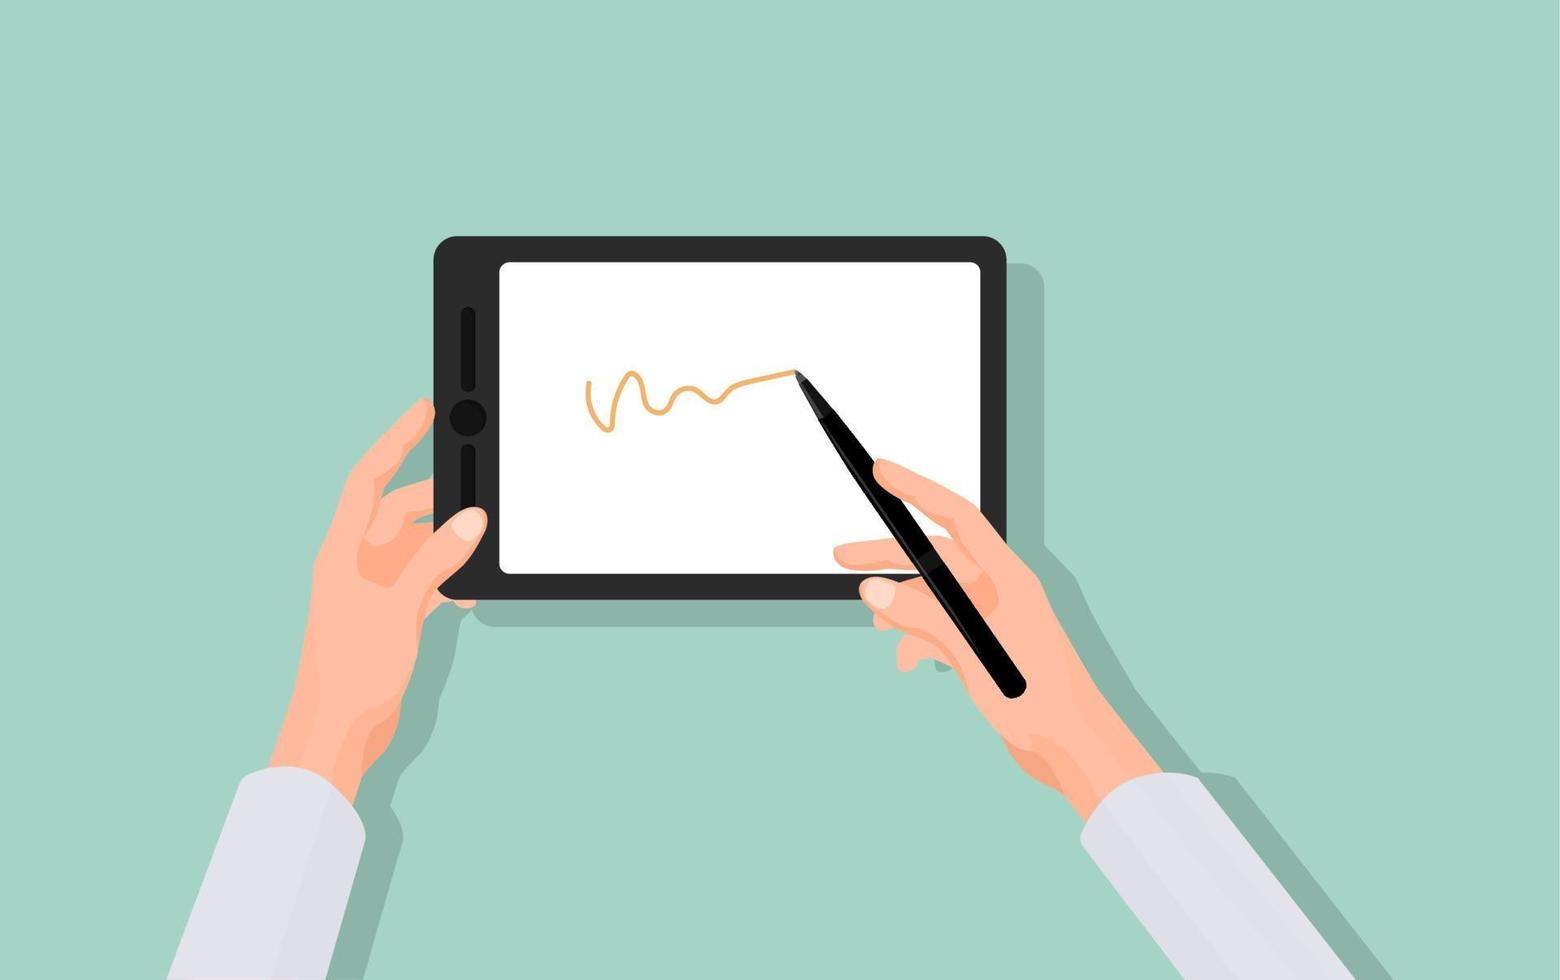
\includegraphics[width=0.3\textwidth]{graphics/signature}};
            \begin{scope}[on background layer]
                \node[l, label={[above]Registro do usuário},](left-c){};
            \end{scope}
            \begin{scope}[on background layer]
                \node[r,label={[above]Autenticação do usuário}](right-c)
                [right= 0.01cm of left-c]{};
            \end{scope}
            
            \node[s](reg-ext) at (0, 2){Extração de recursos dinâmicos};
            \node[s](reg-calc)[below=0.2cm of reg-ext]
            {Cálculo de características estatísticas};
            \node[s](reg-creat)[below=0.2 of reg-calc]
            {Criação de modelo de assinatura};
            \node [c, fit= (reg-ext) (reg-calc) (reg-creat)](reg-c){};
            
            \node[s](auth-ext) at (5, 2){Extração de recursos dinâmicos};
            \node[s](auth-calc)[below=0.2cm of auth-ext]
            {Cálculo de características estatísticas};
            \node [c, fit= (auth-ext) (auth-calc)](auth-c){};
            
            \node[db][below=0.75cm of reg-c](storage){Armazenamento de usuários e
            modelos};
            
            \node[s][below=1cm of auth-c](module){Módulo de autenticação}
            \node[s][below=1cm of module](parser){Analisador de modelos}
            
            \node[s, text width=3cm](interface2) at (2.5, -7){Interface do usuário};
            
            \node[t, yshift=-0.2cm][above=0.5cm of interface2];
            
            \draw[thick, ->](signature.west) -| (reg-c.north);
            \draw[thick, ->](signature.east) -| (auth-c.north);
            \draw[thick, ->](reg-c.south) -- (storage.north);
            \draw[thick, ->](auth-c.south) -- (module.north);
            \draw[thick](storage.east) -- (3, -4.7) -- (3, -5.5) -- (5, -5.5)
            edge[->] (parser.south);
            
            \draw[thick, ->](parser.north) -- (module.south);
        
        \end{tikzpicture}
    \end{adjustbox}
    \floatfoot{Adaptado de \cite{baca2011}}
\end{figure}

A autenticação pode ser realizada com base em assinaturas estáticas ou dinâmicas.
No estado estático, apenas a imagem digital da assinatura está disponível,
geralmente conhecida como \textit{off-line}.
Já no modo dinâmico, as assinaturas são obtidas utilizando uma mesa
digitalizadora ou um \textit{display} de computador sensível à caneta,
comumente chamado de \textit{on-line}\cite{navaz2016}.

É comum examinar a altura máxima, comprimento horizontal, relação de aspecto e
número de levantamentos de caneta de uma amostra de assinatura.
Essas medidas consideram o ângulo da caneta, velocidade, pressão,
forma, sequência e outros aspectos de assinaturas manuscritas\cite{dewangan2015}.

